\chapter{TINJAUAN PUSTAKA}

% Ubah konten-konten berikut sesuai dengan isi dari tinjauan pustaka
\section{Hasil penelitian/perancangan terdahulu}

\subsection{A Robust Dead-Reckoning Pedestrian Tracking System with Low Cost Sensors.}

Munculnya perangkat seluler pribadi dengan sensor berbiaya rendah, seperti akselerometer dan kompas digital, telah menjadikan \emph{Dead Reckoning} (DR) 
pilihan yang menarik untuk indoor pelacakan pejalan kaki. Dalam makalah ini, mengusulkan \emph{Dead Reckoning} (DR) yang kuat sistem pelacakan pejalan kaki di atas akses komersial tersebut, 
set sensor BLE yang mampu \emph{Dead Reckoning} (DR). Metode yang diusulkan mengeksploitasi fakta bahwa, beberapa sistem \emph{Dead Reckoning} (DR), 
dibawa oleh pejalan kaki yang sama, memiliki perpindahan relatif yang stabil sehubungan dengan pusat gerak, dan karenanya satu sama lain. 
Kami pertama-tama merumuskan tugas pelacakan yang kuat sebagai maksimum umum posteriori masalah fusi sensor, dan kemudian kami mempersempitnya menjadi sederhana prosedur perhitungan 
dengan asumsi tertentu. Sebuah prototipe dilaksanakan dan dievaluasi dengan sistem benchmark yang mengumpulkan kebenaran dasar secara efisien dan 
akurat. Dalam praktis testbed dalam ruangan, skema yang diusulkan telah menunjukkan kuat kinerja pelacakan, dengan pengurangan kesalahan
pelacakan rata-rata hingga 73,7 persen, dibandingkan dengan metode pelacakan \emph{Dead Reckoning} (DR) tradisional \parencite{Jin2011}.

\subsection{AI-IMU Dead-Reckoning.}

Makalah ini mengusulkan pendekatan baru untuk inersia hanya \emph{Dead Reckoning} (DR) untuk kendaraan beroda yang dibangun di atas jaringan saraf 
dalam untuk secara dinamis mengadaptasi parameter filter Kalman. Kami telah menunjukkan fakta-fakta berikut. Dimungkinkan untuk mendapatkan 
hasil yang sangat akurat hanya dengan menggunakan \emph{Inertial Measurement Unit} (IMU) berbiaya sedang, berkat penggunaan filter Kalman yang menggabungkan persamaan \emph{Inertial Measurement Unit} (IMU) 
standar dengan informasi samping tentang dinamika kendaraan beroda. Algoritma ini bersaing dengan metode berbasis visi, meskipun hanya \emph{Inertial Measurement Unit} (IMU) 
yang digunakan (dan tidak ada satu pun sensor lain, seperti GNSS). Jaringan saraf dalam adalah alat yang ampuh untuk adaptasi dinamis parameter penyetelan filter Kalman (matriks kovarians kebisingan). 
Di luar jaring saraf dalam, menilai kovarians pengukuran dengan benar secara dinamis memungkinkan filter Kalman mencapai kinerja yang jauh lebih baik, dan ini membuka jalan untuk fusi dengan sensor lain. 
Subjek generalisasi, dan terutama bagaimana arsitektur jaringan dapat digunakan kembali dalam aplikasi serupa, dibiarkan untuk penelitian di masa depan, karena penyetelan \emph{Convolutional Neural Network} (CNN) 
mewakili dalam dirinya sendiri bidang penelitian saat ini.Yang mengatakan, kode yang kami buat tersedia untuk umum dapat digunakan apa adanya, dan disesuaikan dengan kendaraan lain. 
Selain itu, seperti yang disebutkan dalam Bagian VI-E, artikel tersebut membuktikan bahwa adaptasi kovarians dinamis memainkan peran besar untuk lokalisasi yang akurat, 
dan aturan adaptasi rekayasa praktis sederhana dapat dikejar alih-alih yang berbasis \emph{Artificial Intelligence} (AI) \parencite{Brossard2020}.

\section{Teori Dasar}

\subsection{Dead Reckoning (DR)}
Perhitungan mati (\emph{Dead Reckoning}) adalah proses memperkirakan posisi saat ini dengan memproyeksikan heading dan kecepatan dari masa lalu yang diketahui posisi. 
Heading dan kecepatan digabungkan menjadi sebuah gerakan Vektor V1 mewakili perubahan posisi dari A posisi yang diketahui, P0, ke posisi yang diperkirakan, P1. 
Akurasi dari perkiraan ini dapat dikutip sebagai elips kepercayaan diri yang rata-rata populasinya ada di elips 95 persen dari waktu. Sumbu elips ditentukan oleh 
keakuratan deteksi heading dan pengukuran kecepatan. Pengguna yang berpindah dari titik P0 ke titik P1 dapat diilustrasikan berada dalam elips kepercayaan 95 persen 
berpusat pada P1 dengan sumbu AB, ditentukan oleh heading akurasi sensor, dan CD, ditentukan oleh sensor kecepatan ketepatan.
Untuk melakukan \emph{Dead Reckoning}, kalian memerlukan informasi berikut: [1] Posisi awal: Ini adalah posisi objek atau orang yang diketahui di awal perjalanan.
[2] Heading: Ini adalah arah di mana objek atau orang bepergian, biasanya diukur dalam derajat dari utara.
[3] Jarak yang ditempuh: Ini adalah jarak yang telah ditempuh objek atau orang dari posisi awal.

% Contoh input gambar dengan format *.jpg
\begin{figure} [ht] \centering
  % Nama dari file gambar yang diinputkan
  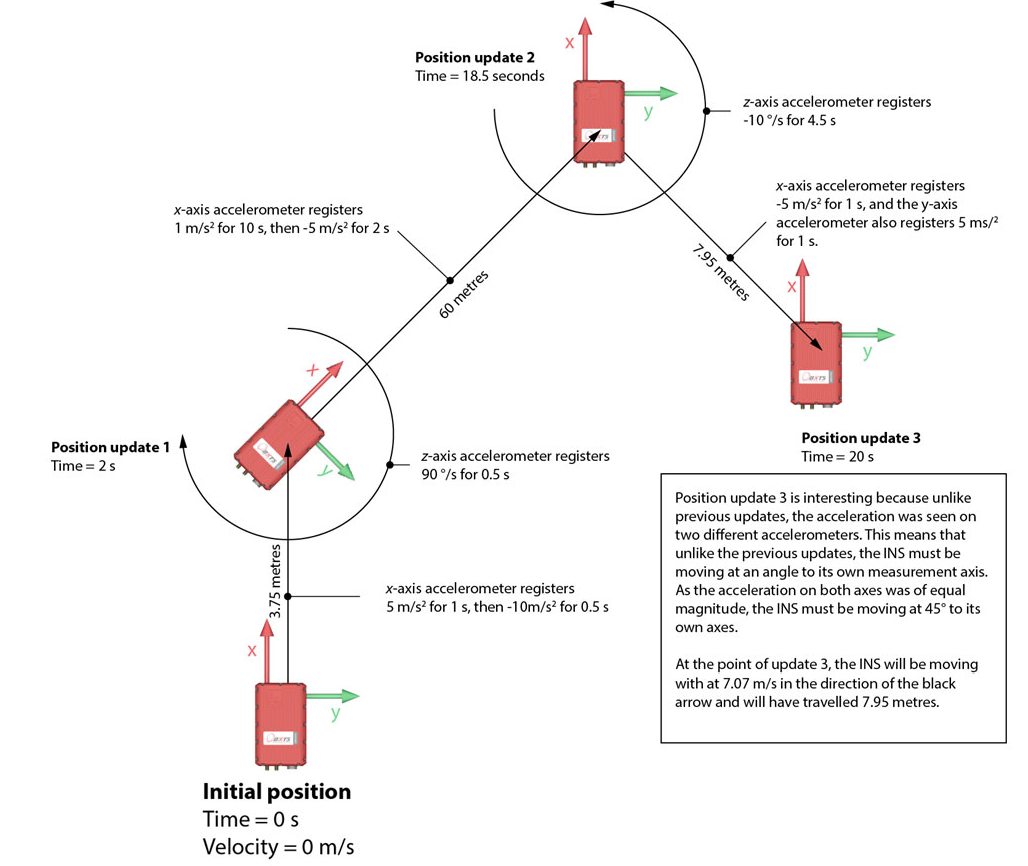
\includegraphics[scale=0.45]{gambar/Dead-reckoning-INS.png}
  % Keterangan gambar yang diinputkan
  \caption{\emph{Inertial navigation} menggunakan \emph{Dead Reckoning} \parencite{oxts2020-dr}}
  % Label referensi dari gambar yang diinputkan
  \label{fig:DR}
\end{figure}

\subsection{Convolutional Neural Network (CNN)}

Jaringan saraf convolutional (CNN) adalah jenis jaringan saraf tiruan yang dirancang khusus untuk pengenalan dan pemrosesan gambar. Itu terdiri dari beberapa lapisan neuron buatan 
(juga dikenal sebagai "unit" atau "node"), yang masing-masing bertanggung jawab untuk mempelajari fitur atau atribut tertentu dari data input. Salah satu fitur utama \emph{Convolutional Neural Network} adalah penggunaan
lapisan konvolusional, yang bertanggung jawab untuk mempelajari fitur data masukan secara otomatis. Lapisan ini menggunakan satu set filter, juga dikenal sebagai kernel atau bobot, 
untuk mendeteksi pola dalam data. Filter diterapkan ke data input menggunakan proses yang disebut konvolusi, yang melibatkan menggeser filter melintasi data input dan melakukan perkalian 
berdasarkan elemen dengan elemen dalam input. Keluaran yang dihasilkan disebut peta fitur, yang merepresentasikan keberadaan fitur tertentu dalam data masukan. \emph{Convolutional Neural Network} dapat dilatih untuk 
mengenali pola dan mengklasifikasikan gambar dengan menyesuaikan bobot filter di lapisan konvolusional. Mereka biasanya digunakan dalam tugas klasifikasi gambar, seperti mengenali objek 
dalam gambar atau mengklasifikasikan gambar ke dalam kategori yang berbeda. Mereka juga berhasil dalam tugas-tugas lain seperti pemrosesan bahasa alami dan pengenalan suara.

Faktanya, \emph{Convolutional Neural Network} memiliki lebih banyak opsi yang menyediakan banyak peluang untuk bahkan mengurangi parameter semakin banyak, dan pada saat yang sama 
mengurangi beberapa efek samping. Salah satu opsi ini adalah hanya berasumsi bahwa node layer berikutnya memiliki banyak tumpang tindih dengan tetangga mereka dengan melihat daerah.
Kita bisa memanipulasi tumpang tindih dengan mengendalikan langkah, menunjukkangambar 7x7 yang diberikan. Jika kita memindahkan filter satu node setiap kali, kita hanya dapat 
memiliki output 5x5. Perhatikan bahwa output dari tiga matriks kiri, memiliki tumpang tindih (dan tiga tengah satu bersama-sama dan tiga yang benar juga). Namun, jika kita bergerak
dan buat setiap langkah 2, maka outputnya akan menjadi 3x3. Meletakkan sederhananya, tidak hanya tumpang tindih, tetapi juga ukuran output akan menjadi berkurang. Untuk melakukan 
\emph{Dead Reckoning} menggunakan \emph{Convolutional Neural Network}, jaringan perlu dilatih pada kumpulan data input yang terdiri dari posisi kendaraan sebelumnya dan data sensorik yang dikumpulkan selama periode waktu 
tertentu, dan label output yang sesuai yang mewakili posisi kendaraan saat ini. \emph{Convolutional Neural Network}  kemudian akan dapat membuat prediksi tentang posisi kendaraan saat ini berdasarkan data input baru 
yang terdiri dari posisi kendaraan sebelumnya dan data sensorik yang dikumpulkan pada titik waktu tertentu.Ada banyak aplikasi potensial untuk menggunakan \emph{Convolutional Neural Network}  untuk perhitungan mati, 
termasuk kendaraan otonom, drone, dan robot seluler lainnya.Kemampuan untuk secara akurat memperkirakan posisi kendaraan saat ini berdasarkan posisi sebelumnya dan data sensorik dapat 
sangat penting untuk navigasi dan lokalisasi di lingkungan di mana sinyal GPS mungkin tidak tersedia atau tidak dapat diandalkan \parencite{Albawi2017}. 

\subsection{Accelerometers}

Akselerometer adalah otomatis alat untuk mengukur akselerasi, mendeteksi dan mengukur getaran (vibration) dan akselerasi pengukuran karena tubuh (inclination). Akselerometer dapat 
digunakan untuk mengukur getaran pada mobil, mesin, bangunan, dan keamanan Instalasi. Akselerometer juga dapat diterapkan pada mengukur peralatan elektronik, seperti 3 dimensi permainan, 
mouse komputer dan telepon dan gempa bumi kegiatan dan dapat digunakan untuk keperluan multimedia seperti VOD (Video on Demand) yang video tersebut menggunakan gerakan 3D dan objek 3D 
dapat diubah menjadi gambar seperti JPG yang memiliki fungsi kontinu dari intensitas cahaya di sebuah dimensi. Hadir dalam bentuk sirkuit sederhana untuk perangkat elektronik besar. 
Meskipun penampilannya sederhana, akselerometer terbuat dari berbagai bagian dan bekerja dalam banyak hal, dua di antaranya adalah \emph{Capacitance Accelerometer} 
dan \emph{Piezoelectric Acceleromete} \parencite{Randell2003}. 

Untuk sistem akselerometer multi-sensor, pengklasifikasi pohon keputusan digunakan sebagai algoritma klasifikasi. Ukuran jendela tetap 1 sec dan laju pengambilan sampel 20Hz diadopsi untuk sistem ini seperti yang dijelaskan sebelumnya. Untuk pengklasifikasi, mean, var, 
dan \emph{Spectral Energy} diadopsi sebagai fitur karena kemampuan pengenalannya yang lemah. Dua kombinasi fitur masing-masing digunakan untuk pengklasifikasi pohon keputusan: Hanya rata-rata
dan kombinasi mean dan var. Untuk sistem akselerometer sensor tunggal, ukuran jendela tetap 0,5 sec dan frekuensi pengambilan sampel 50Hz diadopsi, karena sistem sensor tunggal lebih 
sensitif terhadap frekuensi pengambilan sampel di bawah 50Hz. Pengklasifikasi dan fitur-fiturnya dipilih berdasarkan studi yang ditentukan Akselerometer sering kali dilengkapi dengan 
rentang pengukuran yang dapat diprogram. Mereka biasanya memiliki minimum rentang pengukuran gaya ±2 g dan naik ke rentang pengukuran gaya ±24 g. Namun memilih rentang pengukuran yang 
tinggi tidak berarti itu akan menjadi pilihan ideal untuk setiap tugas. Ini adalah karena mengonfigurasi akselerometer ke rentang pengukuran yang lebih besar mengurangi presisi 
akselerometer. Karena itu, jika lebih penting bagi suatu tugas untuk dapat mengukur pengukuran yang luas rentang, maka akselerometer akan dikonfigurasi ke rentang pengukuran tertinggi.

\subsection{Magnetometers}

Modul kompas elektronik 3-sumbu sedang dirancang untuk tujuan penginderaan magnetik medan rendah yang memiliki antarmuka digital, untuk tujuan memberikan informasi judul untuk proyek 
mikrokontroler. Sensor ringkas ini biasanya cocok dengan proyek-proyek kecil seperti UAV dan sistem navigasi robot. Sensor sebenarnya mengubah segala jenis medan magnet menjadi output 
tegangan diferensial pada 3 sumbu. Perubahan tegangan ini adalah nilai output digital mentah, yang dapat digunakan untuk tujuan menghitung heading atau merasakan medan magnet yang datang 
dari berbagai arah. Pertumbuhan pasar kompas elektronik 3 sumbu sangat bergantung pada pertumbuhan pasar otomotif dan kedirgantaraan dan pertahanan secara keseluruhan secara global. 
Magnetometer digunakan dalam berbagai aplikasi, termasuk navigasi, pemetaan medan geomagnetik, dan deteksi logam. Dalam sistem navigasi, magnetometer 3 sumbu dapat digunakan untuk 
mengukur medan magnet bumi dan menentukan orientasi perangkat relatif terhadap kutub utara magnet bumi. Ini berguna untuk menentukan arah atau arah perjalanan kendaraan atau perangkat, 
terutama dalam situasi di mana sinyal GPS tidak tersedia atau tidak dapat diandalkan.

Terlepas dari banyak faktor pendorong, pasar kompas elektronik 3-sumbu diperkirakan akan menunjukkan menyusut dan fluktuasi tingkat pertumbuhan karena adanya teknologi GPS sebagai 
pengganti aplikasi serupa yang terkait dengan navigasi. Tidak adanya perangkat keras tambahan untuk e-compass atau kompas navigasi bertindak sebagai faktor penahan untuk pasar kompas 
elektronik 3-sumbu global. Pengurangan paket sensor untuk tujuan mengintegrasikannya secara efisien ke dalam produk elektronik portabel telah secara portentous mendorong pertumbuhan 
pasar kompas elektronik 3-sumbu dalam beberapa waktu terakhir dan akan menciptakan peluang yang signifikan untuk kompas elektronik 3-sumbu di tahun-tahun mendatang. Ada beberapa jenis 
magnetometer, termasuk fluxgate, efek hall, dan magnetometer yang dipompa secara optik. Magnetometer Fluxgate menggunakan gulungan kawat yang dikelilingi oleh inti feromagnetik. Ketika 
medan magnet hadir, inti termagnetisasi, yang menyebabkan perubahan resistansi kawat. Magnetometer efek hall menggunakan magnetometer tipis, konduktor datar yang diposisikan dalam medan 
magnet. Ketika arus dilewatkan melalui konduktor, dihasilkan tegangan yang sebanding dengan kekuatan medan magnet. Magnetometer yang dipompa secara optik menggunakan laser untuk mengukur 
penyerapan cahaya oleh spesies atom atau molekul untuk menentukan kekuatan medan magnet.

\subsection{Gyroscope}
Giroskop adalah perangkat yang dipasang ke bingkai dan dapat merasakan kecepatan sudut jika itu bingkai adalah rotasi. Ada beberapa kelas giroskop, tergantung pada operasi fisik dan 
teknologi yang melibatkan. Giroskop dapat berdiri sendiri atau digunakan untuk sesuatu sistem yang kompleks, seperti Inertial Measurement Unit (IMU), gyrocompass, sistem referensi judul 
sikap dan sistem navigasi. Untuk mengukur efek Koriolis, giroskop MEMS mengandung massa bergetar yang bergetar di sepanjang drive sumbu. Getaran sekunder diinduksi 
dengan sumbu indera tegak lurus yang menggantikan massa darinya jalur asli ketika giroskop diputar. Prinsip kerja giroskop di mana rotasi di sekitar sumbu masing-masing. 
Giroskop memperkenalkan kapasitansi berubah untuk mendeteksi perpindahan ini. Berbasis pada ini, kecepatan sudut IMU dapat diukur dan dengan mengintegrasikan sinyal, kita dapat memperoleh
orientasi \parencite{Passaro2017}.

Giroskop struktur bergetar mengandung massa mesin mikro yang terhubung ke rumah luar oleh satu set mata air. Rumah luar ini terhubung ke papan sirkuit tetap oleh set pegas ortogonal 
kedua. Massa terus menerus didorong sinusoidal di sepanjang set pegas pertama. Setiap rotasi sistem akan menginduksi percepatan Koriolis dalam massa, mendorongnya ke arah set pegas 
kedua. Ketika massa diusir dari sumbu rotasi, massa akan didorong tegak lurus dalam satu arah, dan ketika didorong kembali ke arah sumbu rotasi, ia akan didorong ke arah yang 
berlawanan, karena gaya Koriolis yang bekerja pada massa.

